\documentclass{article}

\usepackage[polish]{babel}
\usepackage[T1]{fontenc}
\usepackage{tabularx}
\usepackage{amsfonts}
\usepackage{amsmath}
\usepackage{mathtools}
\usepackage{enumitem}
\usepackage{graphicx}

\pagestyle{headings}

\begin{document}

\begin{titlepage}
    \title{Obliczenia Naukowe \\ 
    \large lista 1}
    \author{Mateusz Tofil}
    \maketitle
\end{titlepage}

\section{Zadanie 1}

\subsection{Opis zadania}

Jest to powtórka zadania z listy poprzedniej - listy 1 zadania 5. Jedyna różnica jaka występuje, to usunięcie z  \(x_4\) ostatniej cyfry tj. 9. i z \(x_5\) usunąc ostatnią 7.

\subsection{Metoda rozwiązania}

Metoda niczym się nie różni od wcześniejszego zdaniaz  wcześniejszej liczby. Dane wejśćiowe są tylko inne - a dokładniej tylko \(x_4\) i \(x_5\). Rozwiązanie znajduję się w pliku \texttt{zad1.jl} i jest dokłądną duplikacją kodu z zadania 5 z poprzedniej listy ze zmienionymi danymi wejściowymi.

\subsection{Otrzymane wyniki}

Tabele poniżej przedstawiając sumy obliczone tak jak w zadaniu 5 z listy 1, natomiast lekko zmienionymi wartościami na wejśćiu. Wyniki przedstawione dla arytmetyki \texttt{Float64} i \texttt{Float32}.

\begin{table}[h!]
    \centering
    \begin{tabular}{|l|l|l|l|l|}
     \hline
     podpunkt & sumy z listy 2 & sumy z listy 1\\
     \hline
     \(a\) & -0.004296342739891585 & 1.0251881368296672e-10  \\ 
     \(b\) & -0.004296342998713953 & -1.5643308870494366e-10 \\
     \(c\) & -0.004296342842280865 & 0.0 \\
     \(d\) & -0.004296342842280865 & 0.0 \\
     \hline
    \end{tabular}
    \caption{Porównanie sum z poprzedniej listy i obecnej dla \texttt{Float64}}
    \label{table:1}
\end{table}

\begin{table}[h!]
    \centering
    \begin{tabular}{|l|l|l|}
     \hline
     podpunkt & suma z listy 2 & suma z listy 1 \\
     \hline
     \(a\) & -0.3472038161889941 & -0.3472038161853561  \\ 
     \(b\) & -0.3472038162872195 & -0.3472038162872195 \\
     \(c\) & -0.5 & -0.5 \\
     \(d\) & -0.5 & -0.5 \\
     \hline
    \end{tabular}
    \caption{Wyniki dla \texttt{Float32}}
    \label{table:2}
\end{table}

\subsection{Wnioski}

Zmiana wartości liczby, rzędu nawet \(2^{-10}\) wpływa znacząco na wyniki ostateczny. Niewielkie zmiany spowodowały duże względne odkształcenia wyników, zatem możemy stwierdzić, że zadanie jest źle uwarunkowane.

\section{Zadanie 2}

\subsection{Opis zadania}

Należało narysować funckję \(f(x) = e^x ln (1 + e^{-x})\) w conajmniej dwóch rożnych program do rysowania wykresu, zbadać faktyczną granicę funkcji i porównać z otrzymanymi wykresami.

\subsection{Metoda rozwiązania}

Funkcje \(f(x)\) wpisać do programu umożliwiającego rysowanie wykresów. Programy, które wybrałem do narysowania funkcji \(f(x)\) to: WolframAplha, Grapher oraz postanowiłem napisać programy przedstawiający wykresy w języku programowania Python z wykorzystaniem biblioteki matplotlib in numpy

\subsection{Otrzymane wyniki}

W programie Grapher należało wpisać funkcję w wyznaczone miejsce. Następnie przeskalować oś x, wykonując następujące czynności: Viev > Frame Limit ... i zmienić skalowanie.Na stronie WolframAplha należało wpisać \texttt{plot <funkcja> from -5 to 40}. Program napisany w pythonie znajduję się w pliku o ścieżce \texttt{./zad2/plotpython.py}

\begin{figure}[h!]
    \centering
    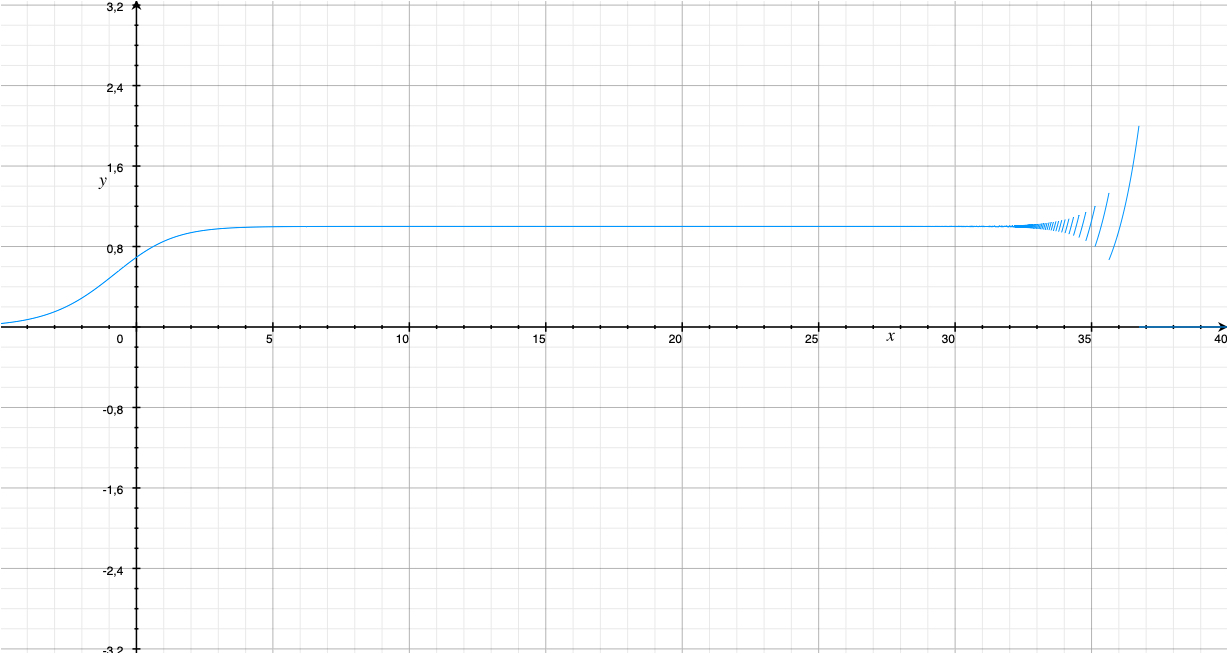
\includegraphics[width=12cm]{./zad2/wykresGrapher.jpg}
    \caption{Wykres funkcji \(f(x)\) w programie Grapher}
    
    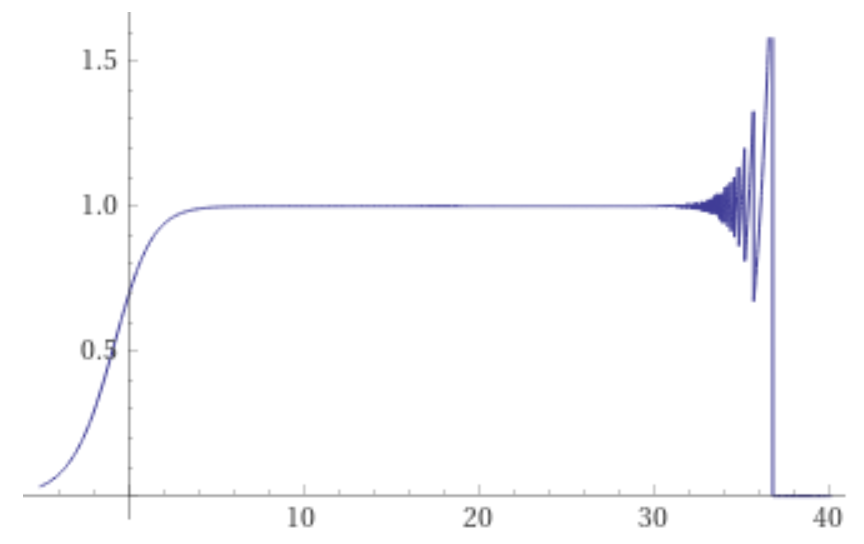
\includegraphics[width=12cm]{./zad2/wykresWolfram.png}
    \caption{Wykres funkcji \(f(x)\) w programie WolframAplha}    
\end{figure}

\begin{figure}
    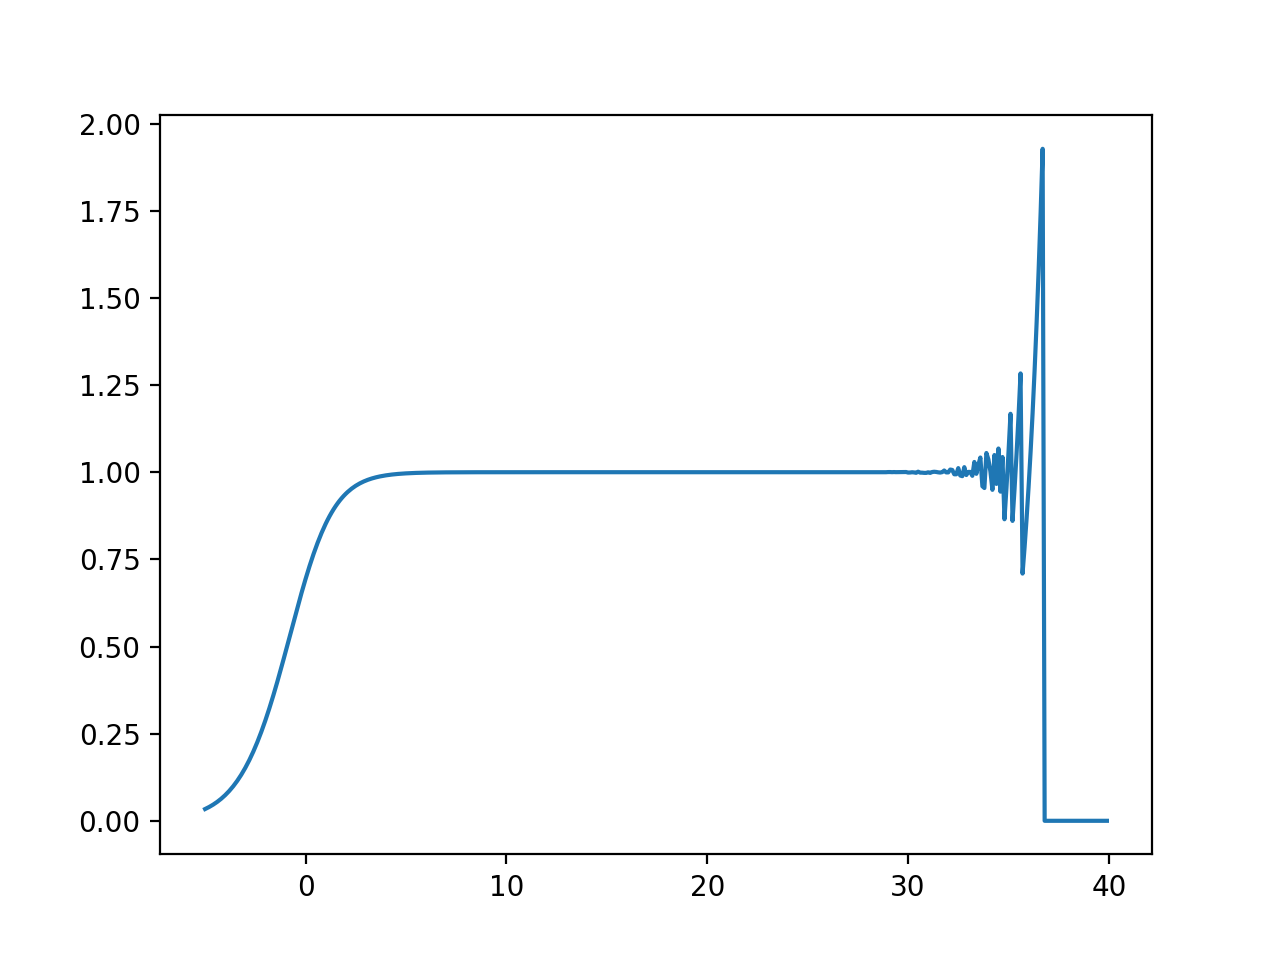
\includegraphics[width=12cm]{./zad2/wykresPython.png}
    \caption{Wykres funkcji \(f(x)\) w języku Python z wykorzystamiem biblioteki matplotlib}
\end{figure}

Obliczmy teraz granicę funkcji:

\begin{multline}
    \lim_{x \to \infty}{e^x \ln(e^{-x}+1) = \lim_{x \to \infty}{\frac{e^x \ln(e^{-x} + 1)e^{-x}}{e^{-x}}}} = \lim_{x \to \infty}{\frac{\ln(e^{-x}+1)}{e^{-x}}} \stackrel{H}{=} \\ \stackrel{H}{=} \lim_{x \to \infty} {\frac{\frac{d}{dx} \ln(e^{-x} + 1)}{\frac{d}{dx} e^{-x}}} = \lim_{x \to \infty}{\frac{-\frac{e^{-x}}{e^{-x}+1}}{-e^{-x}}} = \lim_{x \to \infty} {\frac{1}{e^{-x}+1} = 1} 
\end{multline}

Jak łatwo zauważyć, granica funkcji, którą obliczyliśmy powyżej nie pokrywa się z granicą funkcji odczytując ją z wykresu. Na wykresie granica funkcji dąży do 0 natomiast z matematycznego punktu widzenia dąży do 1. Powyżej argumnetów powyżej 30 obserwujemy, że wykresy zaczynają pokazywać nieprawidłowe wyniki.

\subsection{Wnioski}

Wartości \(e^{-x}\) dla każdego następnego argumentu zbliżając się do epsilona maszynowego, po przekroczeniu epsilona, funkcja spada do zera. Przed przekroczeniem epsiolona maszynowego, funkcja dąży do jedynki, tak jak powinna.

\begin{table}[h!]
    \centering
    \begin{tabular}{|l|l|l|}
    \hline
    wykładnik & \(exp(wykladnik)\) & \(exp(wykladnik) - epsilon \)\\
    \hline
    30 & 9.357622968840175e-14 & 9.335418508347672e-14\\
    31 & 3.442477108469977e-14 & 3.4202726479774736e-14\\
    32 & 1.2664165549094176e-14 & 1.2442120944169144e-14\\
    33 & 4.658886145103398e-15 & 4.4368415401783664e-15\\
    34 & 1.713908431542013e-15 & 1.4918638266169817e-15\\
    35 & 6.305116760146989e-16 & 4.084670710896676e-16\\
    36 & 2.319522830243569e-16 & 9.907678099325606e-18\\
    \hline
    37 & 8.533047625744066e-17 & -1.3671412866759066e-16\\
    38 & 3.1391327920480296e-17 & -1.90653277004551e-16\\
    39 & 1.1548224173015786e-17 & -2.104963807520155e-16\\
    40 & 4.248354255291589e-18 & -2.1779625066973972e-16\\
     \hline
    \end{tabular}
    \caption{Wartości exp() dla kolejnych argumentów porównanie z epsilonem maszynowym}
    \label{table:3}
\end{table}




% \subsection{Opis zadania}
% \subsection{Metoda rozwiązania}
% \subsection{Otrzymane wyniki}
% \subsection{Wnioski}


\end{document}